\chapter{Weights Table for Higgs Sample}
\section{Windowed re-weighting results}
\label{apdx:window_wgts}
\begin{table}[thb]
    \centering
    \footnotesize
    \makebox[\textwidth]{\begin{tabular}{|c|c|c|c|c|c|c|c|c|c|c|c|c|}
\hline
(100 GeV) & 2-3 & 3-5 & 5-6 & 6-7 & 7-8 & 8-9 & 9-10 & 10-15 & 15-20 & 20-25 & 25-30 & 30-80 \\ \hline
30&0.0572 & 0.1082 & 0.0737 & 0.0686 & 0.0742 & 0.0857 & 0.1015 & 0.1431 & 0.1832 & 0.2573 & 0.4859 & 0.74 \\ \hline
25&0.0531 & 0.1011 & 0.071 & 0.0659 & 0.0734 & 0.083 & 0.1001 & 0.1461 & 0.2169 & 0.3597 & 0.3971 & 0.1964 \\ \hline
20&0.0545 & 0.0913 & 0.0659 & 0.0633 & 0.0713 & 0.084 & 0.1021 & 0.1599 & 0.2889 & 0.3043 & 0.0933 & 0.0481 \\ \hline
15&0.0643 & 0.1118 & 0.0829 & 0.0812 & 0.0948 & 0.113 & 0.1447 & 0.2395 & 0.2847 & 0.0732 & 0.022 & 0.0141 \\ \hline
10&0.0242 & 0.0493 & 0.044 & 0.0529 & 0.0752 & 0.1179 & 0.1896 & 0.1752 & 0.0141 & 0.0028 & 0.0008 & 0.0008 \\ \hline
9&0.0238 & 0.0468 & 0.0465 & 0.0602 & 0.1028 & 0.1791 & 0.2064 & 0.0832 & 0.0066 & 0.0013 & 0.0004 & 0.0003 \\ \hline
8&0.0205 & 0.045 & 0.0592 & 0.0941 & 0.1991 & 0.2324 & 0.1099 & 0.0341 & 0.0031 & 0.0007 & 0.0002 & 0.0001 \\ \hline
7&0.0207 & 0.0478 & 0.076 & 0.1965 & 0.2409 & 0.0787 & 0.0324 & 0.012 & 0.0014 & 0.0003 & 0.0001 & 0.0001 \\ \hline
6&0.0212 & 0.0637 & 0.2502 & 0.2875 & 0.0573 & 0.0205 & 0.0098 & 0.0048 & 0.0007 & 0.0002 & 0.0 & 0.0001 \\ \hline
5&0.014 & 0.0705 & 0.217 & 0.0251 & 0.0083 & 0.0041 & 0.0023 & 0.0014 & 0.0002 & 0.0 & 0.0 & 0.0 \\ \hline
3&0.2708 & 0.2386 & 0.0111 & 0.0037 & 0.002 & 0.0012 & 0.0008 & 0.0006 & 0.0001 & 0.0 & 0.0 & 0.0 \\ \hline
2&0.3757 & 0.0259 & 0.0026 & 0.001 & 0.0006 & 0.0004 & 0.0003 & 0.0001 & 0.0 & 0.0 & 0.0 & 0.0 \\ \hline
\end{tabular}}
\caption{Windowed re-weigthing result for ggZZ samples.}
\end{table}

\begin{table}[thb]
    \centering
    \footnotesize
    \makebox[\textwidth]{\begin{tabular}{|c|c|c|c|c|c|c|c|c|c|c|c|c|c|}
\hline
(100 GeV) & 2-3 & 3-4 & 4-5 & 5-6 & 6-7 & 7-8 & 8-9 & 9-10 & 10-15 & 15-20 & 20-25 & 25-30 & 30-80 \\ \hline
30                       & 0.0013  & 0.0024  & 0.0021  & 0.0035  & 0.003   & 0.005   & 0.01    & 0.0112   & 0.0265    & 0.0764    & 0.1583    & 0.3873    & 0.6233    \\ \hline
25                       & 0.0017  & 0.0028  & 0.0023  & 0.0046  & 0.004   & 0.0063  & 0.0121  & 0.0149   & 0.039     & 0.1193    & 0.2795    & 0.3844    & 0.2218    \\ \hline
20                       & 0.0015  & 0.0044  & 0.0038  & 0.0067  & 0.0065  & 0.0096  & 0.0211  & 0.0256   & 0.0709    & 0.2562    & 0.3658    & 0.1491    & 0.0904    \\ \hline
15                       & 0.0045  & 0.0088  & 0.0075  & 0.015   & 0.0131  & 0.0218  & 0.0448  & 0.06     & 0.1727    & 0.4011    & 0.1484    & 0.0569    & 0.0434    \\ \hline
10                       & 0.0052  & 0.0077  & 0.0092  & 0.0184  & 0.0208  & 0.0464  & 0.0152  & 0.0085   & 0.2471    & 0.0459    & 0.0136    & 0.0058    & 0.0055    \\ \hline
9                        & 0.0054  & 0.0142  & 0.0167  & 0.0378  & 0.0449  & 0.0975  & 0.332   & 0.4022   & 0.2029    & 0.0389    & 0.0122    & 0.0058    & 0.0052    \\ \hline
8                        & 0.0107  & 0.0196  & 0.0252  & 0.0623  & 0.0998  & 0.3037  & 0.187   & 0.2898   & 0.1195    & 0.0255    & 0.0085    & 0.0036    & 0.0042    \\ \hline
7                        & 0.0087  & 0.0226  & 0.0299  & 0.1043  & 0.2057  & 0.2715  & 0.2067  & 0.0905   & 0.0481    & 0.0125    & 0.0047    & 0.0023    & 0.0022    \\ \hline
6                        & 0.0176  & 0.0482  & 0.0882  & 0.0557  & 0.4805  & 0.157   & 0.1003  & 0.0499   & 0.0348    & 0.0108    & 0.0039    & 0.002     & 0.0017    \\ \hline
5                        & 0.029   & 0.1134  & 0.2939  & 0.5247  & 0.1041  & 0.0499  & 0.0397  & 0.025    & 0.0188    & 0.0065    & 0.0026    & 0.0015    & 0.0013    \\ \hline
4                        & 0.0634  & 0.336   & 0.4353  & 0.1231  & 0.001   & 0.0183  & 0.0174  & 0.0129   & 0.0111    & 0.0042    & 0.0015    & 0.0008    & 0.0007    \\ \hline
3                        & 0.1082  & 0.3288  & 0.0725  & 0.0305  & 0.0114  & 0.0086  & 0.009   & 0.0064   & 0.0058    & 0.0022    & 0.0009    & 0.0005    & 0.0004    \\ \hline
2                        & 0.7428  & 0.0912  & 0.0134  & 0.0132  & 0.005   & 0.0042  & 0.0047  & 0.0031   & 0.0028    & 0.0004    & 0.0       & 0.0       & 0.0       \\ \hline
\end{tabular}}
\caption{Windowed re-weigthing result for VBF samples.}
\end{table}
\pagebreak

\section{Sample mass factors for ggZZ and VBF\_ZZ samples}
\label{apdx:mass_wgts}
\begin{table}[]
    \centering
\begin{tabular}{|c|c|c|c|}
\hline
\multicolumn{2}{|c|}{ggZZ} & \multicolumn{2}{c|}{VBF\_ZZ} \\ \hline
Mass (GeV)     & Factor    & Mass (GeV)      & Factor     \\ \hline
200            & 1         & 200             & 1          \\ \hline
300            & 0.8798    & 300             & 0.8731     \\ \hline
500            & 1.1068    & 400             & 0.7873     \\ \hline
600            & 0.7327    & 500             & 0.7106     \\ \hline
700            & 0.6833    & 600             & 0.6361     \\ \hline
800            & 0.6370    & 700             & 0.5754     \\ \hline
900            & 0.6001    & 800             & 0.5217     \\ \hline
1000           & 0.5658    & 900             & 0.4818     \\ \hline
1500           & 0.4769    & 1000            & 0.4257     \\ \hline
2000           & 0.4300    & 1500            & 0.3255     \\ \hline
2500           & 0.4204    & 2000            & 0.2968     \\ \hline
3000           & 0.4256    & 2500            & 0.2898     \\ \hline
               &           & 3000            & 0.2916     \\ \hline
\end{tabular}
\caption{Sample mass re-weighting factors for both signal samples.}
\end{table}

\chapter{Additional Figures}
\pagebreak
\section{GGH Sample Fitting Templates of Background and Signal}
\label{apdx:templates_hist}
\begin{figure}[hbt]
\begin{center}
\subfloat[]{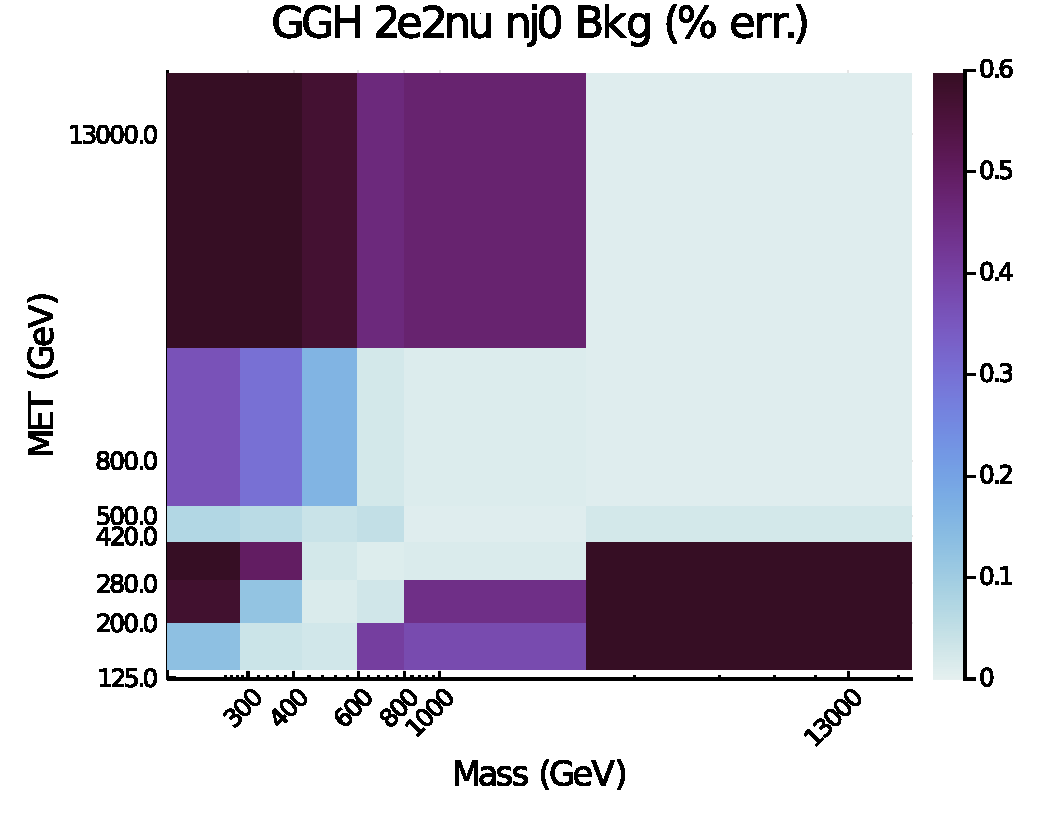
\includegraphics[width=.33\linewidth]{fig/ggZZ_templates/ggZZ_2e2nu_nj0_Bkg.pdf}}
\subfloat[]{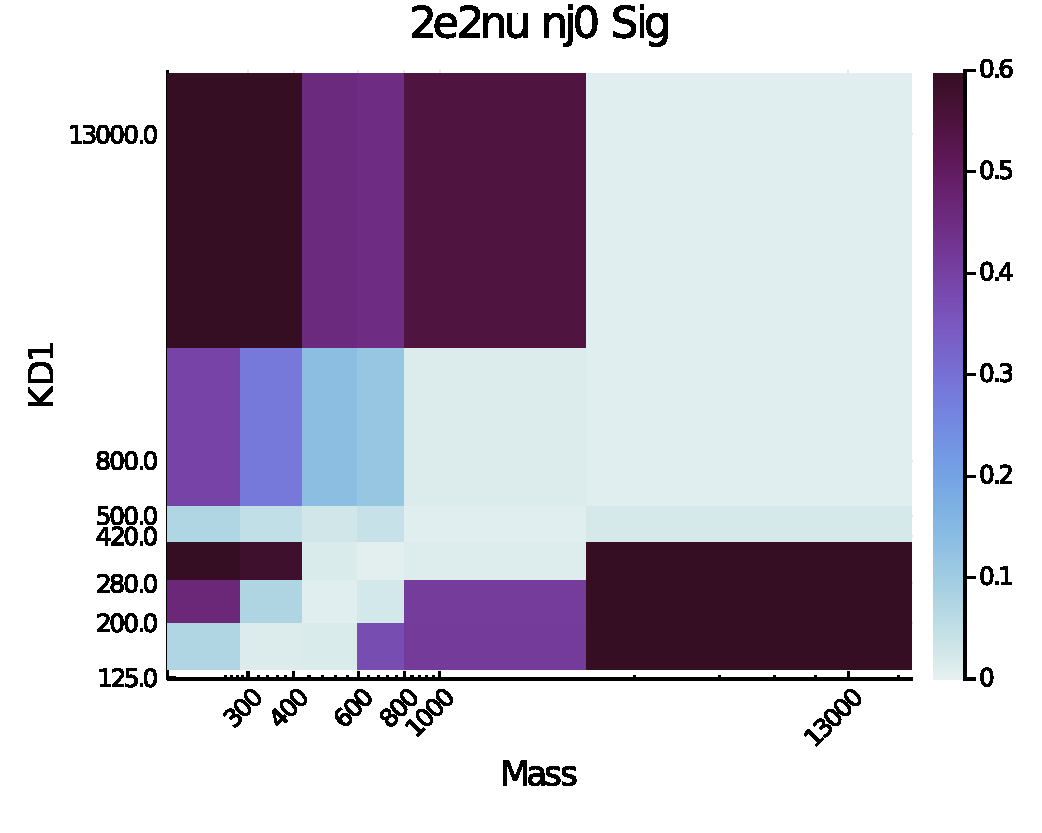
\includegraphics[width=.33\linewidth]{fig/ggZZ_templates/ggZZ_2e2nu_nj0_Sig.pdf}}
\subfloat[]{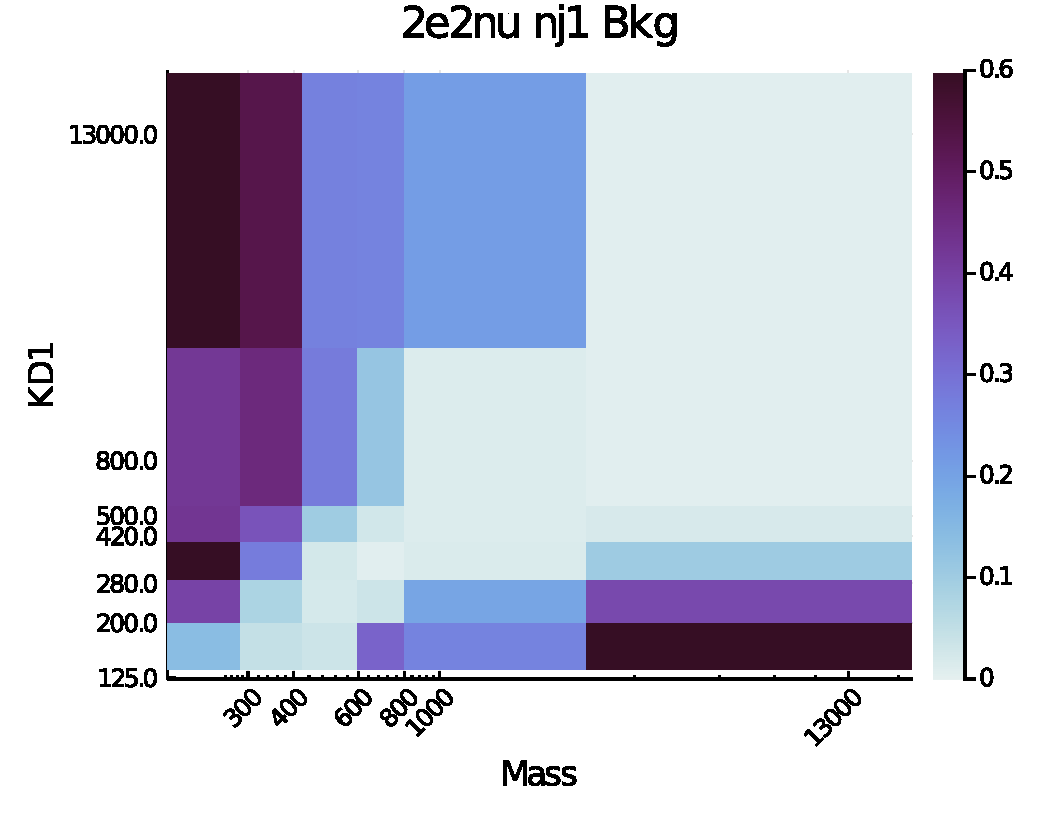
\includegraphics[width=.33\linewidth]{fig/ggZZ_templates/ggZZ_2e2nu_nj1_Bkg.pdf}}\\
\subfloat[]{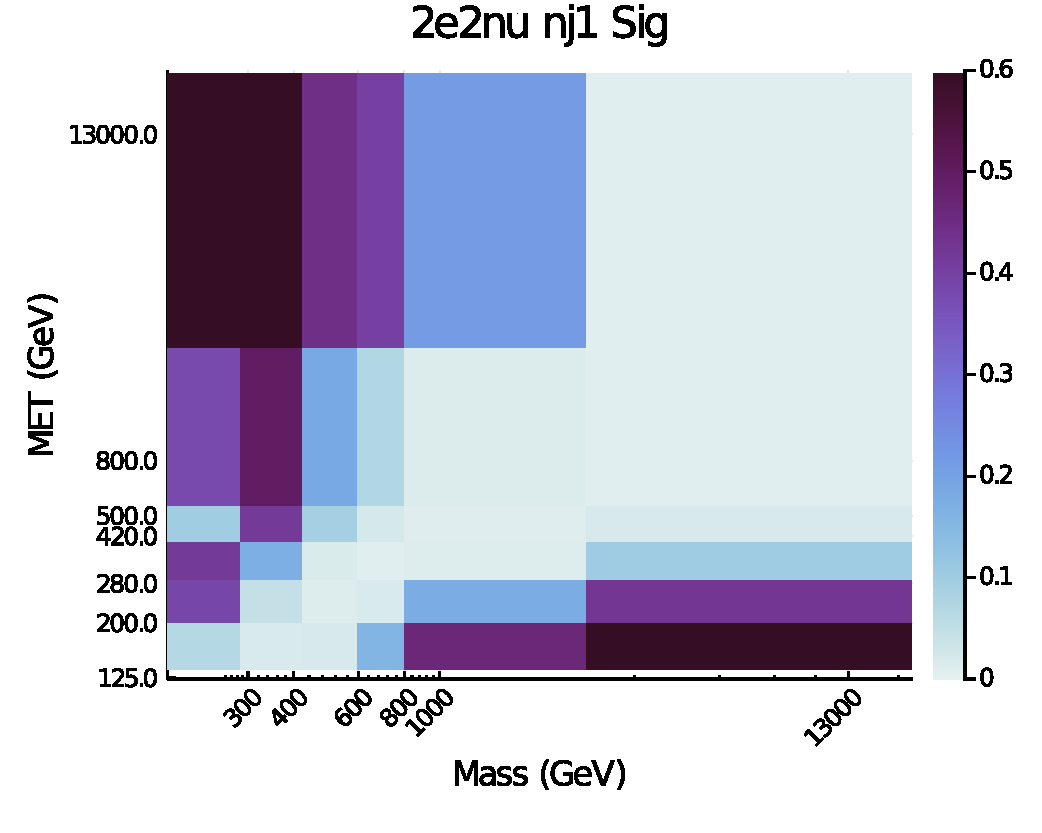
\includegraphics[width=.33\linewidth]{fig/ggZZ_templates/ggZZ_2e2nu_nj1_Sig.pdf}}
\subfloat[]{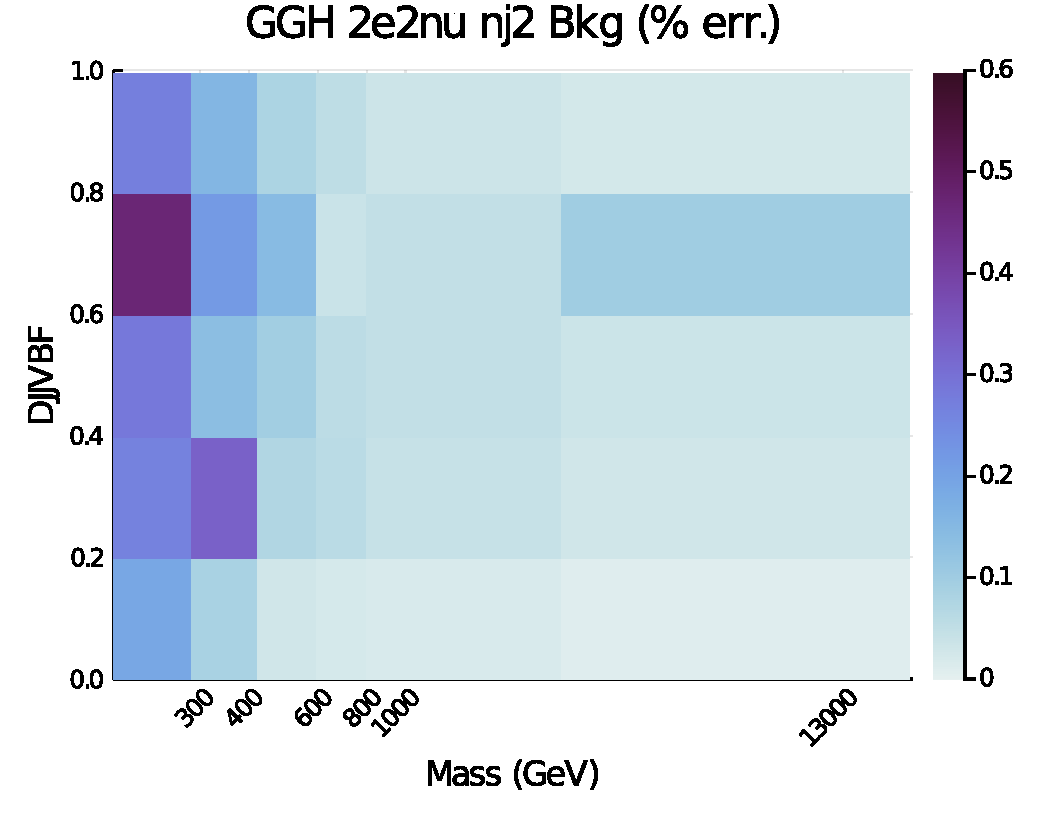
\includegraphics[width=.33\linewidth]{fig/ggZZ_templates/ggZZ_2e2nu_nj2_Bkg.pdf}}
\subfloat[]{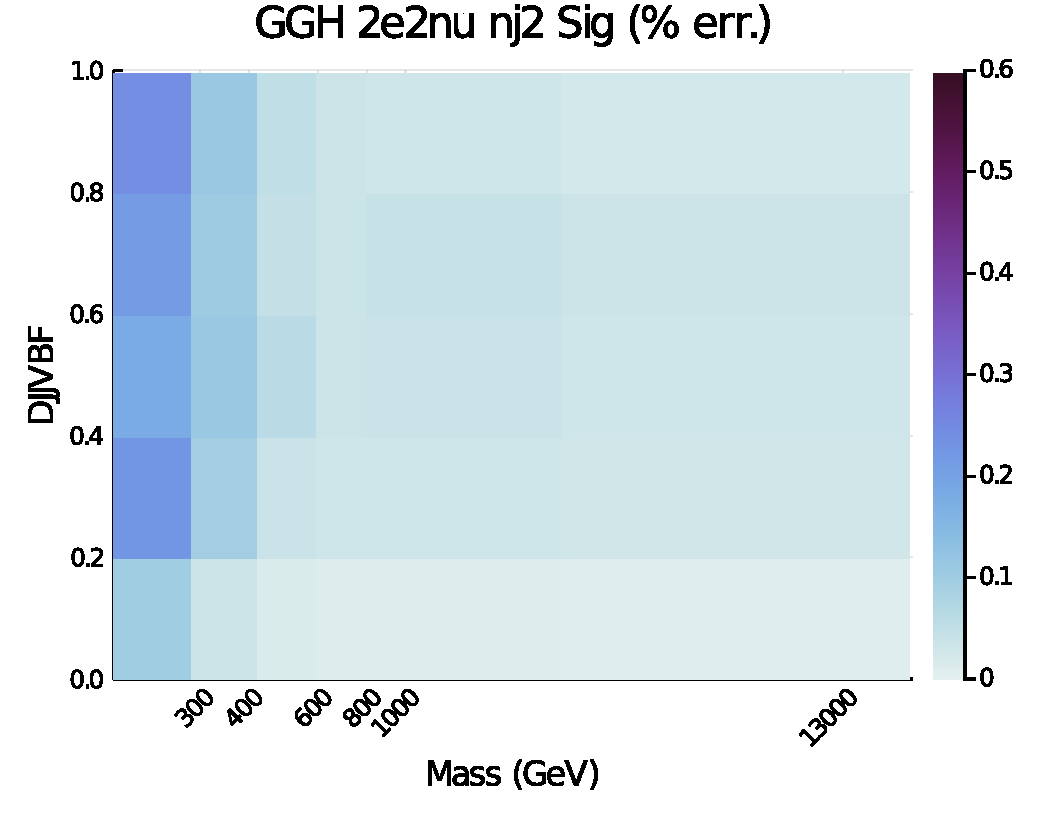
\includegraphics[width=.33\linewidth]{fig/ggZZ_templates/ggZZ_2e2nu_nj2_Sig.pdf}}\\
\subfloat[]{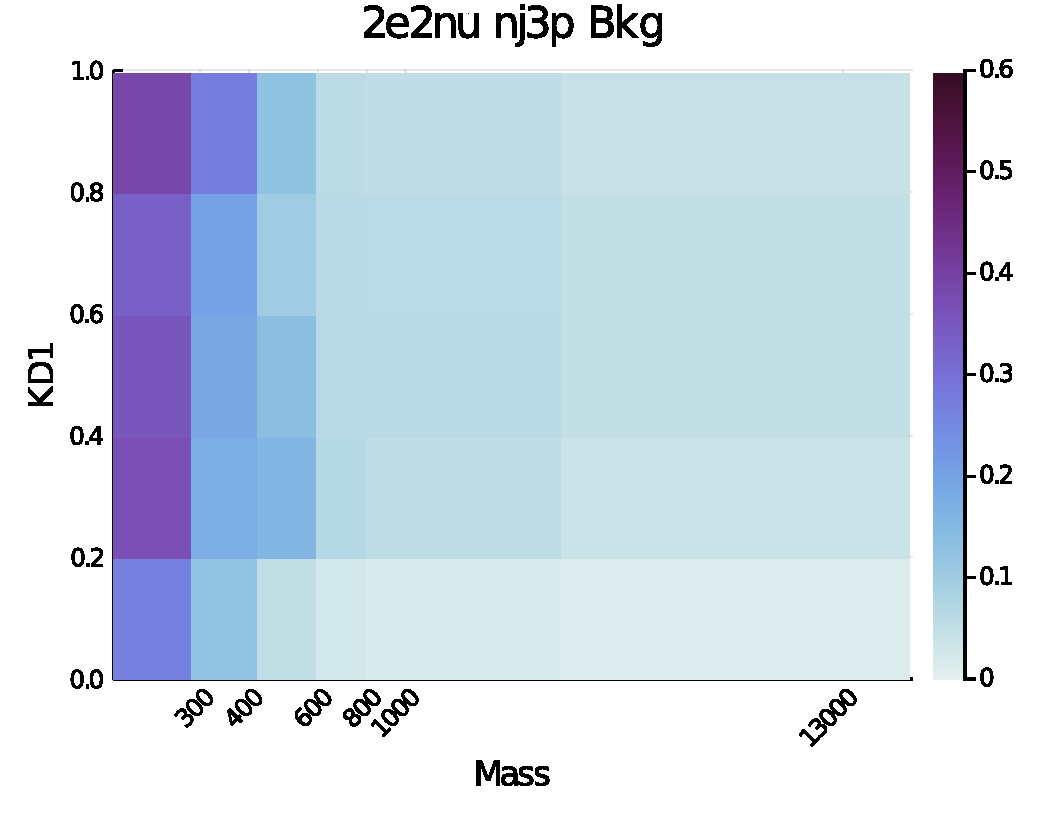
\includegraphics[width=.33\linewidth]{fig/ggZZ_templates/ggZZ_2e2nu_nj3p_Bkg.pdf}}
\subfloat[]{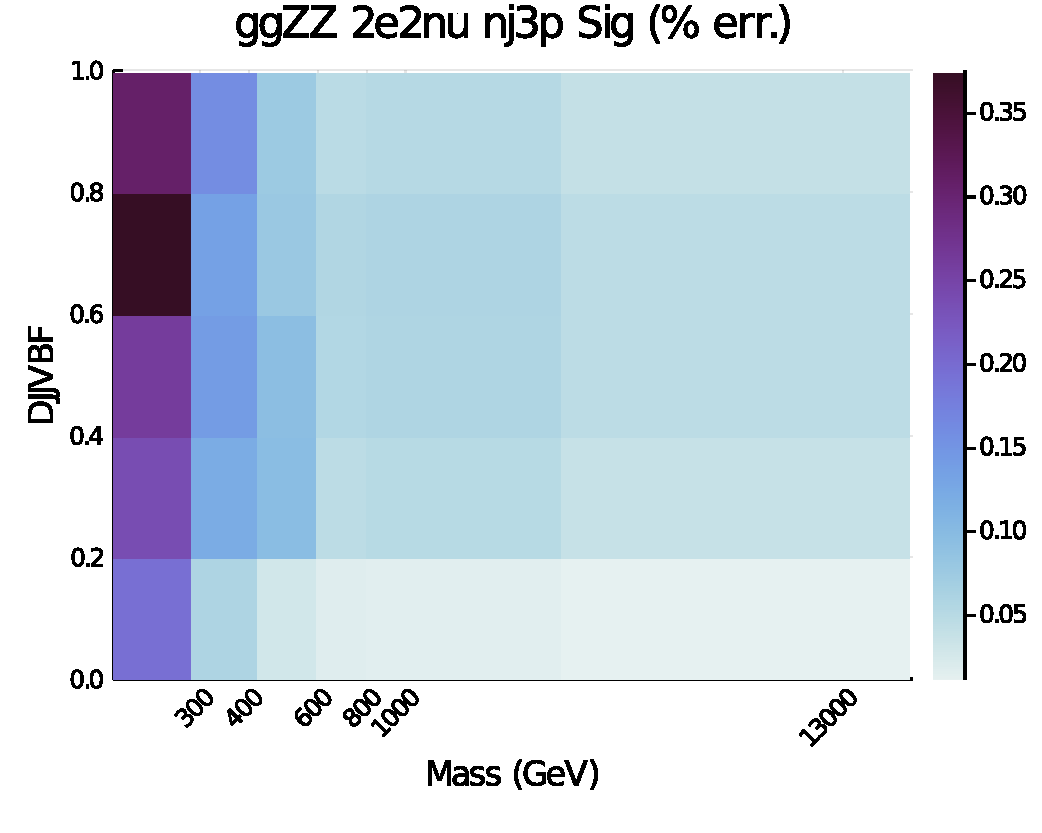
\includegraphics[width=.33\linewidth]{fig/ggZZ_templates/ggZZ_2e2nu_nj3p_Sig.pdf}}
\end{center}
\caption{Iterative sample mass factors obtained (left) and the final combined sample (right)}
\label{fig:LHE_rewgt}
\end{figure}

\begin{figure}[htb]
\begin{center}
\subfloat[]{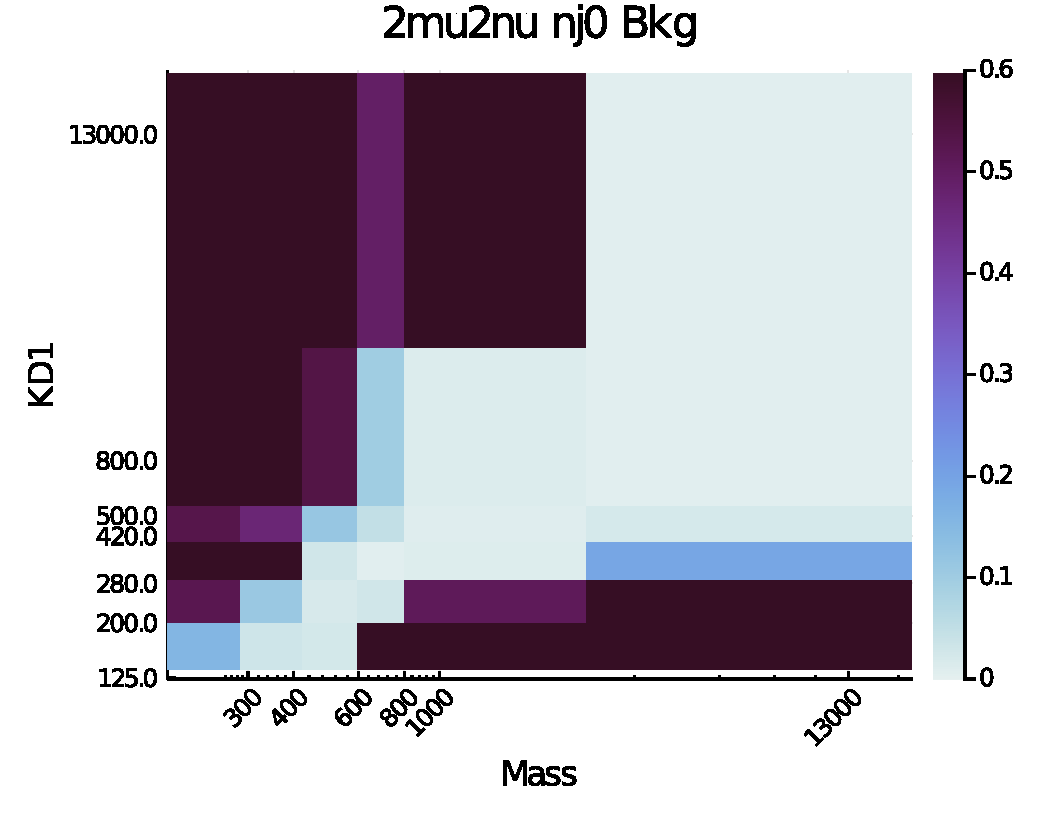
\includegraphics[width=.33\linewidth]{fig/ggZZ_templates/ggZZ_2mu2nu_nj0_Bkg.pdf}}
\subfloat[]{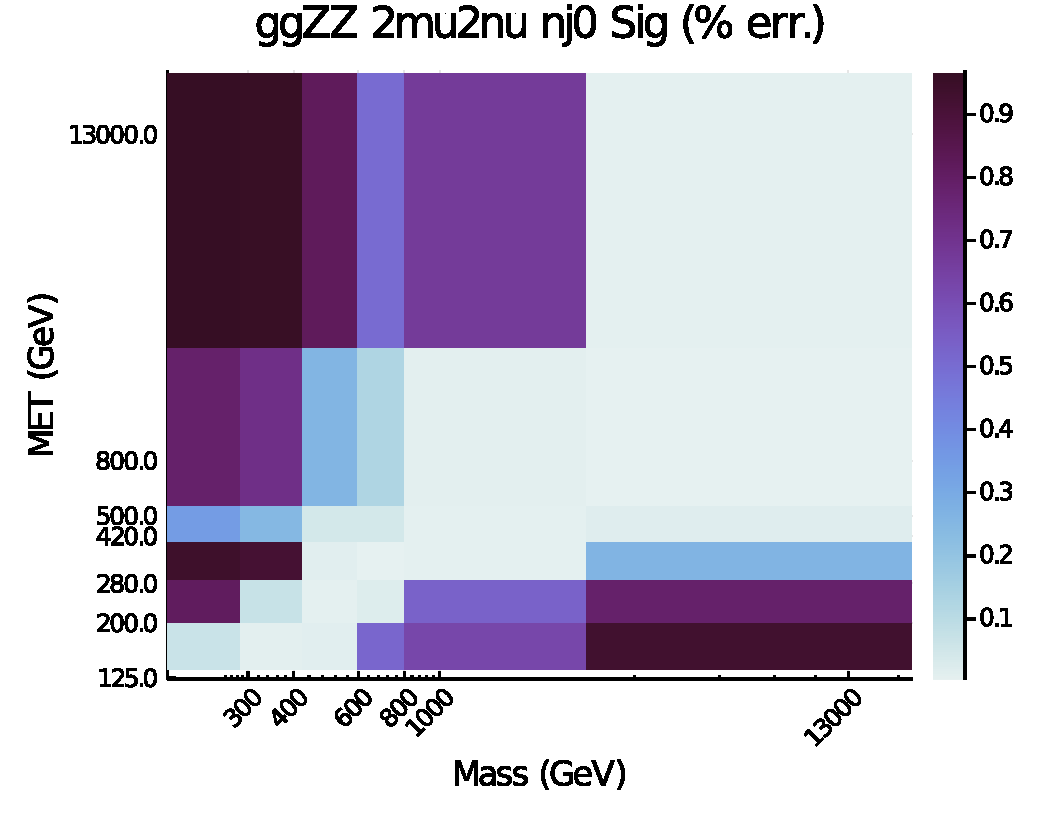
\includegraphics[width=.33\linewidth]{fig/ggZZ_templates/ggZZ_2mu2nu_nj0_Sig.pdf}}
\subfloat[]{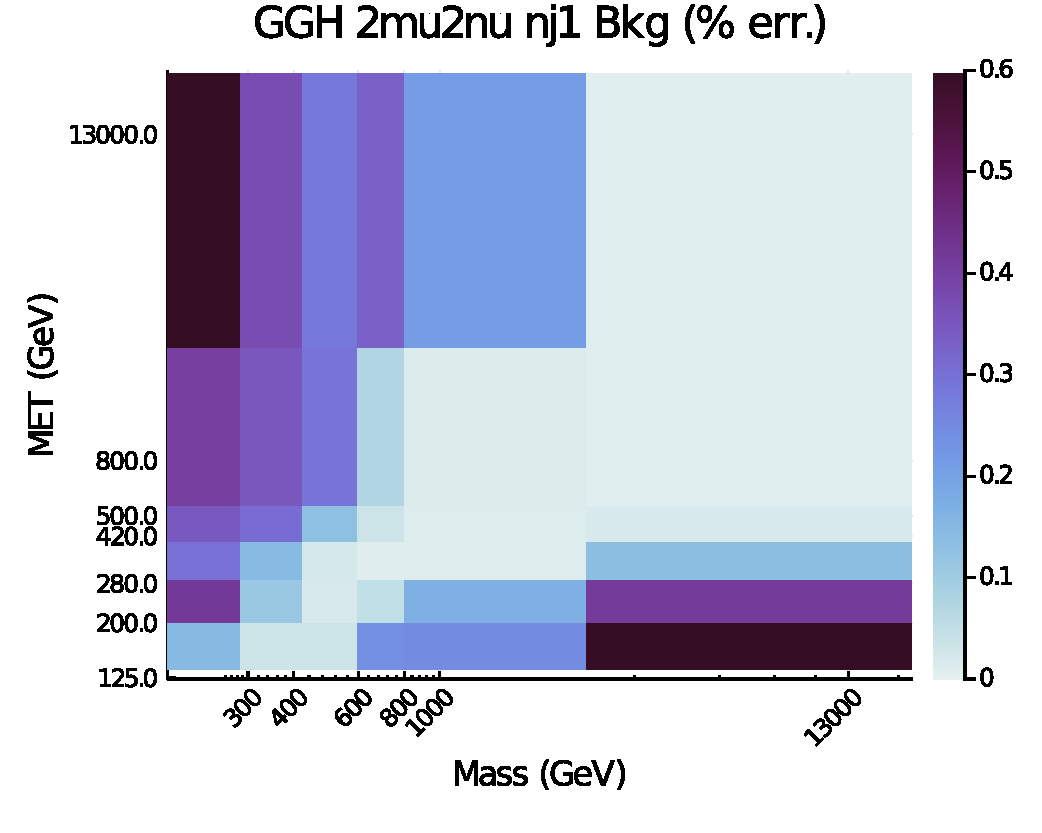
\includegraphics[width=.33\linewidth]{fig/ggZZ_templates/ggZZ_2mu2nu_nj1_Bkg.pdf}}\\
\subfloat[]{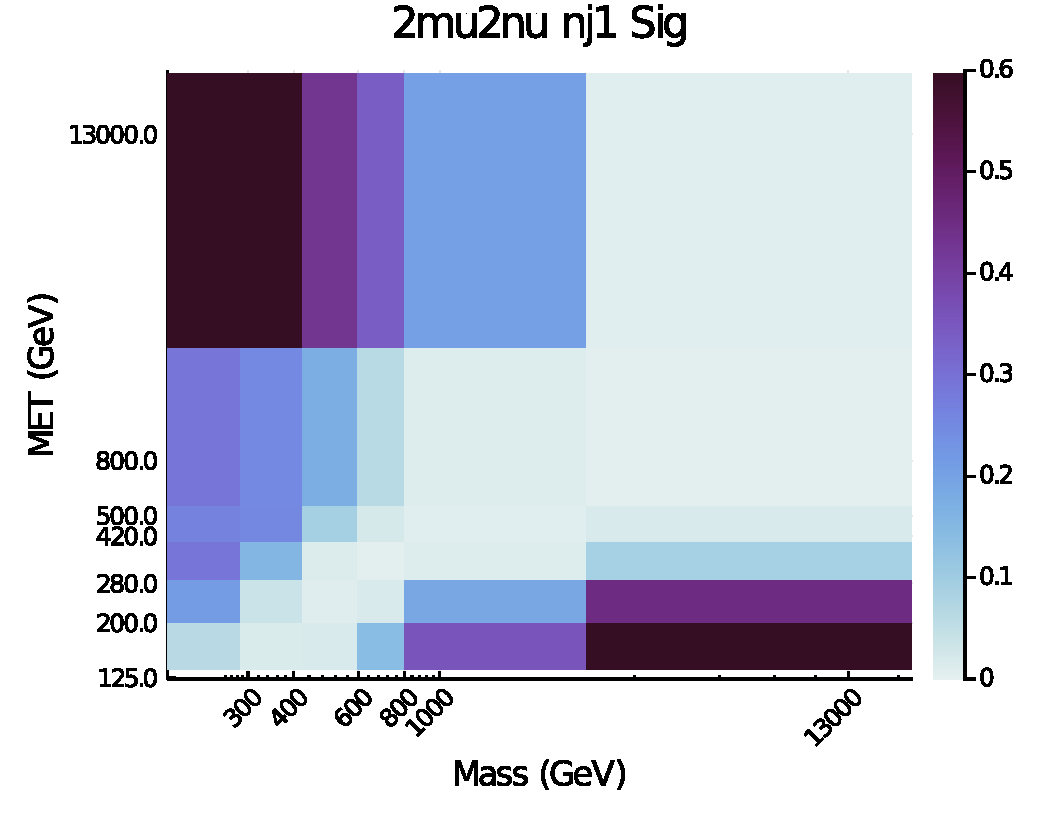
\includegraphics[width=.33\linewidth]{fig/ggZZ_templates/ggZZ_2mu2nu_nj1_Sig.pdf}}
\subfloat[]{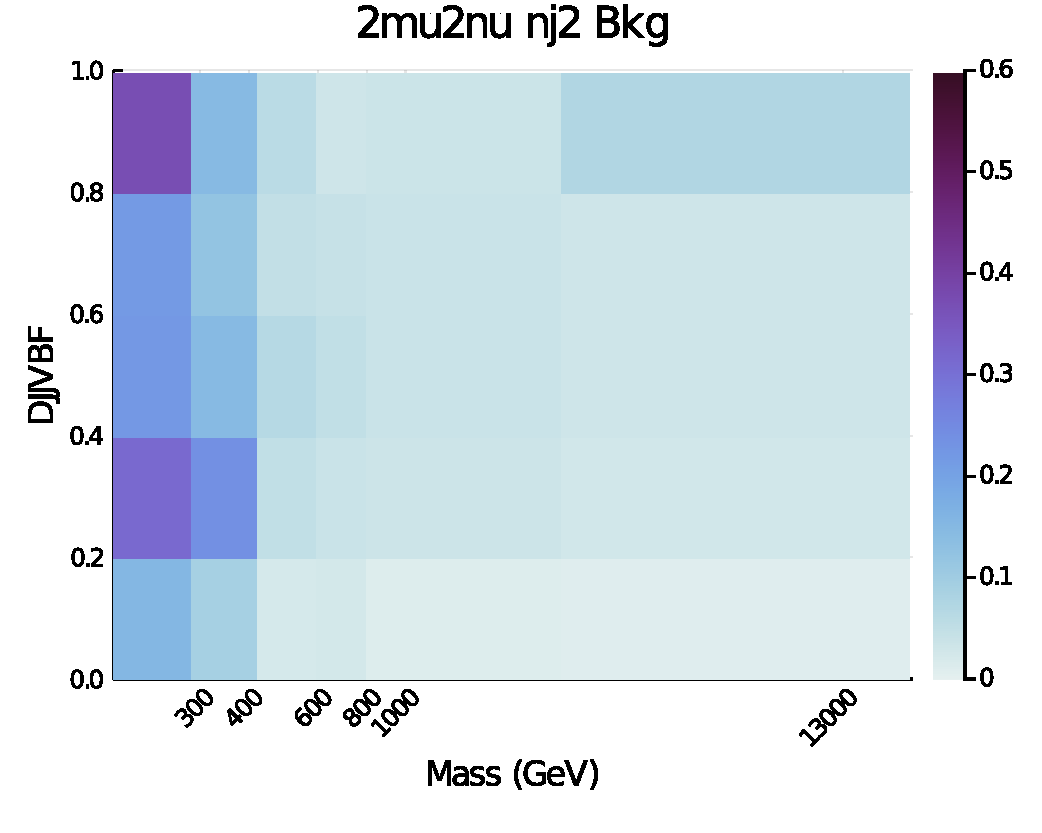
\includegraphics[width=.33\linewidth]{fig/ggZZ_templates/ggZZ_2mu2nu_nj2_Bkg.pdf}}
\subfloat[]{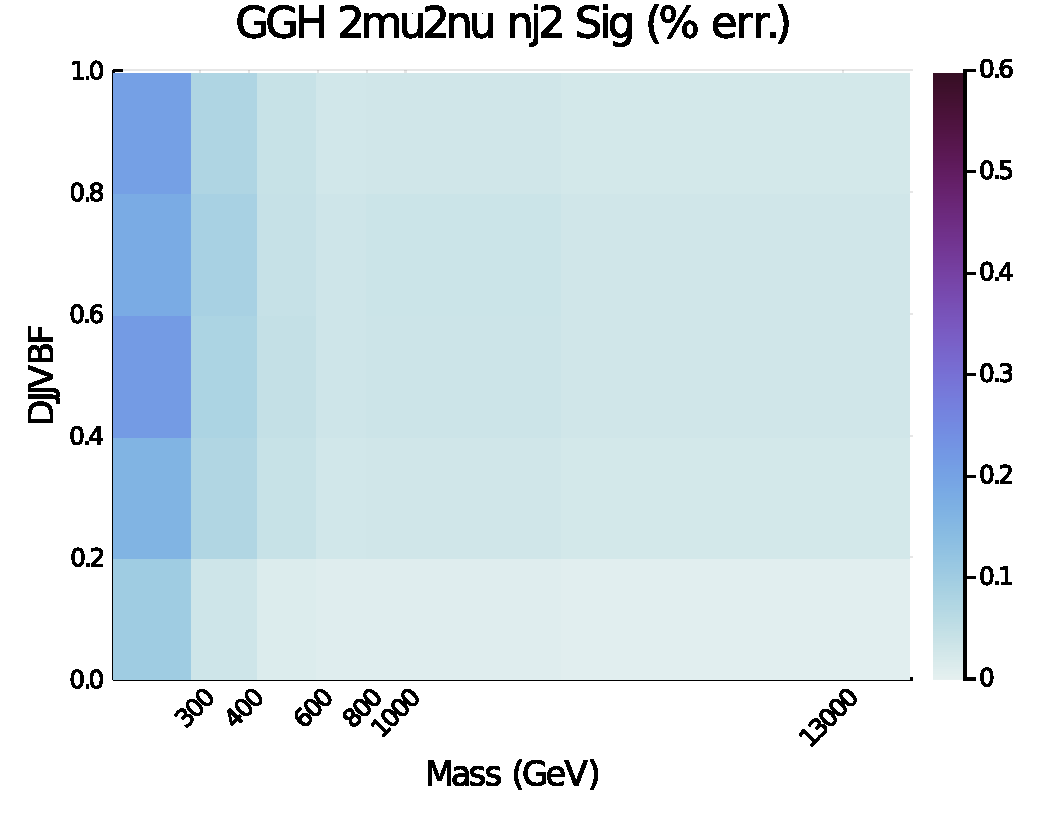
\includegraphics[width=.33\linewidth]{fig/ggZZ_templates/ggZZ_2mu2nu_nj2_Sig.pdf}}\\
\subfloat[]{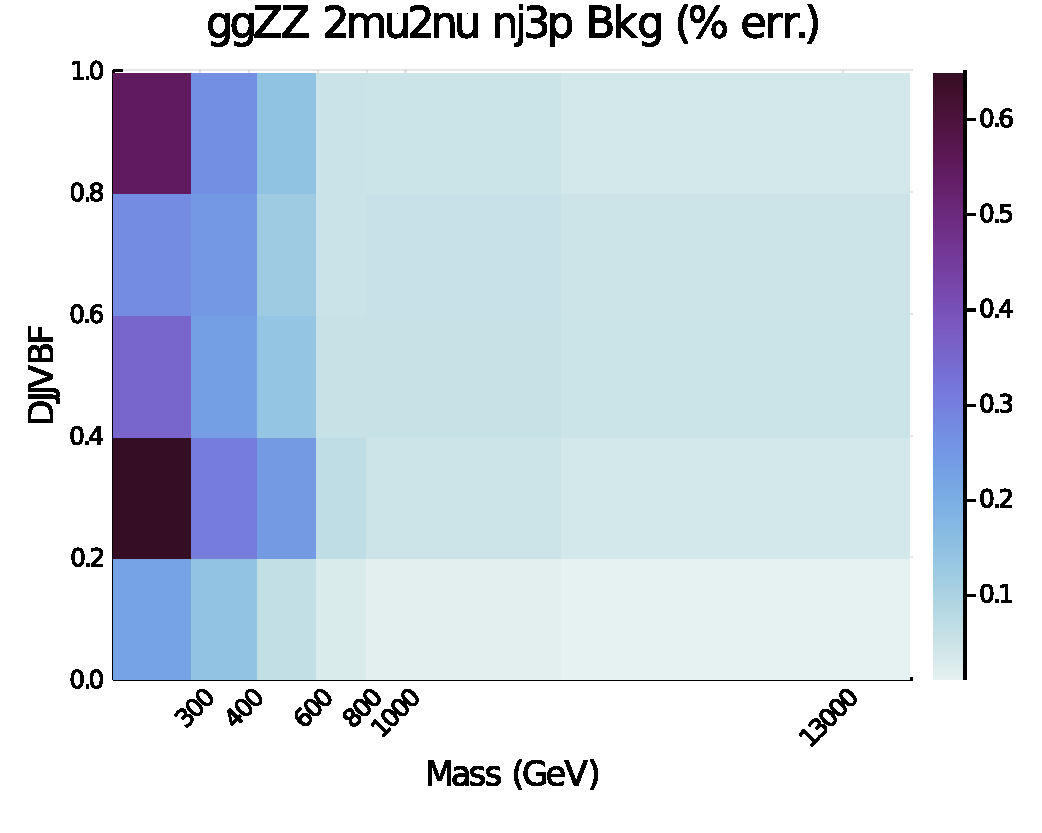
\includegraphics[width=.33\linewidth]{fig/ggZZ_templates/ggZZ_2mu2nu_nj3p_Bkg.pdf}}
\subfloat[]{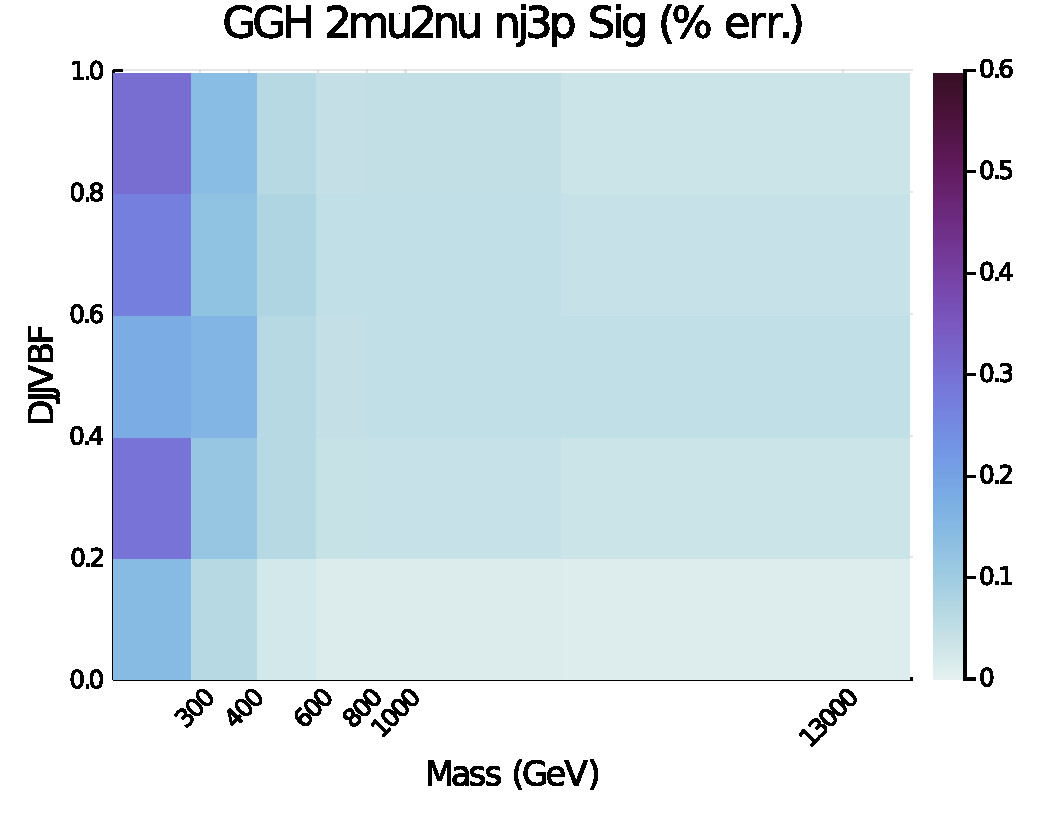
\includegraphics[width=.33\linewidth]{fig/ggZZ_templates/ggZZ_2mu2nu_nj3p_Sig.pdf}}
\end{center}
\caption{Iterative sample mass factors obtained (left) and the final combined sample (right)}
\label{fig:LHE_rewgt}
\end{figure}
